\chapter{Arhitectura}

\paragraph{}
Modelarea unui limbaj reprezint\u a o sarcin\u a extrem de dificil\u a pentru un calculator. Recente progrese \^ in aria Deep Learning au f\u acut posibile diverse dezvolt\u ari \^ in aceast\u a direc\c tie, \^ ins\u a lucrurile sunt departe de a fi rezolvate. Arhitectura folosit\u a pentru construc\c tia chatbot-ului prezentat \^ in aceast\u a lucrare va fi expus\u a precum un bloc de construc\c tii, plec\^ and de la no\c tiunile de baz\u a, p\^ an\u a la arhitectura final\u a.

\section{Re\c tele neurale artificiale}

\paragraph{}
O re\c tea neural\u a artificial\u a (RNA) reprezint\u a o paradigm\u a bazat\u a pe procesare de informa\c tii a c\u arei inspira\c tie provine din sistemul nervos biologic. Precum creierul uman, o RNA este compus\u a dintr-un num\u ar mare de elemente de procesare interconectate (neuroni) lucr\^ and la unison pentru a rezolva diverse probleme. RNA, precum oamenii, \^ inva\c t\u a din exemple. \^ Inv\u a\c tarea \^ in sistemele biologice implic\u a ajustarea conexiunilor sinaptice care exist\u a \^ intre neuroni. Acest principiu se aplic\u a \c si acestor re\c tele.

\paragraph{}
Ca \c si modelare matematic\u a propriu-zis\u a, o RNA poate fi observat\u a \^ in Figura 3.1. Avem o intrare reprezentat\u a \^ in figur\u a de vectorul n-dimensional (x1, x2, x3, x4). Aceast\u a intrare reprezint\u a caracteristicile unui e\c santion care face parte dintr-un set de date. Straturile intermediare se numesc straturi ascunse, iar rolul lor este s\u a produc\u a o abstractizare c\^ at mai complex\u a a datelor de intrare, folosind diverse func\c tii cu activare neliniar\u a. Ultimul strat se nume\c ste strat de ie\c sire, reprezent\^ and eticheta (clasa) vectorului de intrare.

\begin{figure}[H]
\centering
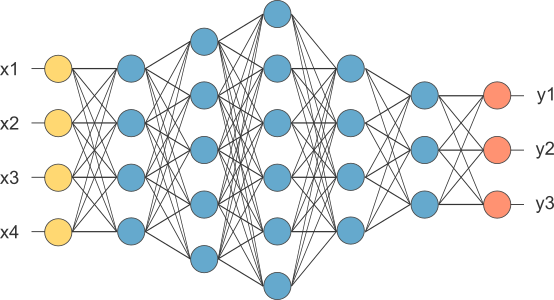
\includegraphics[width=0.7\textwidth]{deep_neural_network}
\caption{Exemplu de re\c tea neural\u a artificial\u a}
\end{figure}

\paragraph{}
Ceea ce de fapt acest tip de re\c tele incearc\u a s\u a inve\c te sunt ponderile dintre straturile sale. Se pleac\u a de la un set de ponderi alese aleator\footnote{Valorile ponderilor sunt deobicei subunitare iar ini\c tializarea este f\u acut\u a urm\^ and diverse principii matematice bine definite. Pentru cazuri simpliste, ini\c tializarea poate fi totu\c si facut\u a folosind o distribu\c tie uniform\u a.} \c si se ajusteaz\u a folosind algoritmul de propagare \^ inapoi a erorii p\^ an\u a c\^and re\c teaua se stabilizeaz\u a. 

\paragraph{}
TO CONTINUE

\section{Re\c tele neurale artificiale recurente}

\paragraph{}
Dup\u a cum se poate observa, o RNA este util\u a atunci c\^ and intrarea este format\u a dintr-un singur element, de exemplu o imagine. Modelarea unui limbaj \^ ins\u a presupune ca intr\u arile s\u a fie fraze. O fraz\u a este format\u a din mai multe elemente (cuvinte), deci o RNA clasic\u a nu poate modela o astfel de intrare. Solu\c tia pentru aceast\u a problem\u a este oferit\u a de re\c telele neurale artificiale recurente (RNAR). Acestea sunt folosite pentru a modela secven\c te unde exist\u a o dependen\c t\u a temporal\u a (fraze, serii de timp). Fiecare intrare curent\u a din secven\c t\u a este condi\c tionat\u a de cele precedente. O astfel de re\c tea se poate observa \^ in Figura 3.2. Straturile ascunse \^ intr-o RNAR au rolul de a p\u astra o captur\u a a tot ceea ce s-a oferit ca intrare p\^ an\u a \^ in momentul curent. Valoarea fiec\u arui strat ascuns curent depinde astfel at\^ at de intrarea curent\u a c\^ at \c si de ie\c sirea stratului ascuns anterior. Putem considera toat\u a aceast\u a modelare ca pe o probabilitate condi\c tionat\u a \( P(x_{n} | x_{1}, x_{2},..., x_{n-1}) \), unde \^ in cazul unei fraze \(x_{1}, x_{2},..., x_{n}\) reprezint\u a cuvintele acesteia. 

\begin{figure}[H]
\centering
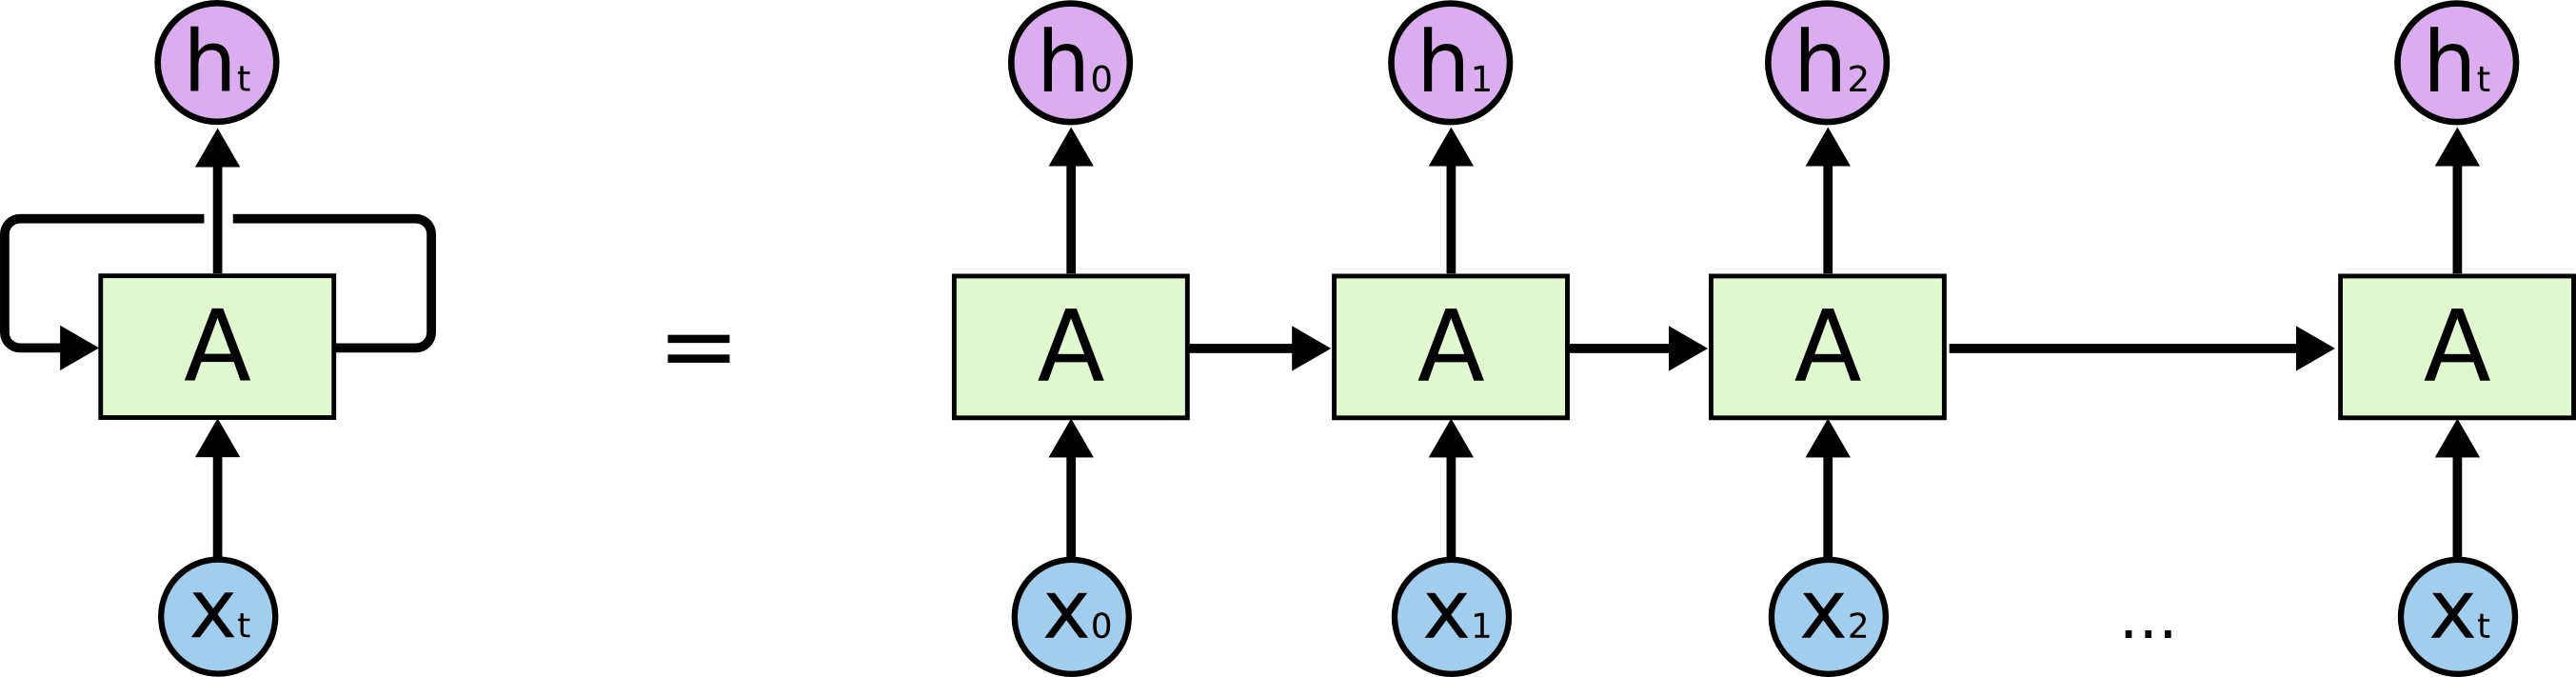
\includegraphics[width=0.9\textwidth]{rnn_network}
\caption{Exemplu de re\c tea neural\u a artificial\u a recurent\u a}
\end{figure}

\paragraph{}
Algoritmul de reglare a ponderilor se nume\c ste propagarea \^ inapoi \^ in timp a erorii. O problem\u a serioas\u a care a ap\u arut odat\u a cu introducerea acestor re\c tele se nume\c ste anularea gradien\c tilor\footnote{vanishing gradients}. \^ In cazul \^ in care secven\c ta de intrare are o lungime mare, informa\c tia nu reu\c se\c ste s\u a se propage \^ in timp deoarece gradientul ponderilor tinde s\u a devin\u a \(0\). Mecanismul care \^ inl\u atur\u a aceast\u a problem\u a se nume\c ste Long Short Term Memory (LSTM). Principiul este ca prin folosirea unor por\c ti de transmitere a informa\c tiei, gradientul s\u a fie stabilizat. Acest mecanism a reprezentat un avans spectaculos pentru Deep Learning, permi\c t\^ and modelarea secven\c tial\u a cu re\c tinere a informa\c tiei pe o perioad\u a \^ indelungat\u a de timp. Ecua\c tiile 3.1 descriu calculele pentru por\c tile LSTM.

\begin{equation}
\begin{split}
f_{t} = \sigma(W_{f}x_{t} + U_{f}h_{t-1} + b_{f})\\
i_{t} = \sigma(W_{i}x_{t} + U_{i}h_{t-1} + b_{i})\\
o_{t} = \sigma(W_{o}x_{t} + U_{o}h_{t-1} + b_{o})\\
c_{t} = f_{t} \circ c_{t-1} + i_{t} \circ \tanh (W_{c}x_{t} + U_{c}h_{t-1} + b_{c})\\
h_{t} = o_{t} \circ \tanh (c_{t})\\
\end{split}
\end{equation}

\paragraph{}
Poarta \(f_{t}\) se nume\c ste poart\u a de uitare (forget gate). Rolul ei este s\u a stabilieasc\u a c\^ at\u a informa\c tie se va uita din trecut. Poarta \(i_{t}\) este poarta de intrare (input gate). Aceasta delimiteaz\u a care este cantitatea de informa\c tie care se p\u astreaz\u a din intrarea curent\u a. Poarta \(o_{t}\) este cea de ie\c sire (output gate). Ea controleaz\u a ce informa\c tie va fi transmis\u a c\u atre ie\c sire. \(c_{t}\) se nume\c ste starea intern\u a a celulei LSTM. Aceasta este calculat\u a ca o combina\c tie \^ intre starea anterioar\u a a celulei, poarta de intrare \c si cea de ie\c sire. \(h_{t}\) reprezint\u a ie\c sirea curent\u a a re\c telei \c si depinde de poarta de ie\c sire \c si starea celulei LSTM. 

\paragraph{}
O RNAN aduce mai aproape ideea de modelare lingvistica, \^ ins\u a se poate observa c\u a aceasta nu permite ca intrare dec\^ at o fraz\u a pe r\^ and. Modelarea dorit\u a \^ in aceast\u a lucrare este o pereche de forma \^ intrebare-r\u aspuns.

\section{Modele Sequence-to-Sequence}

\paragraph{}
Transla\c tia a reprezentat mereu un punct de interes \^ in mediul proces\u arii naturale de limbaj, constituind de altfel o provocare uria\c s\u a de-a lungul ultimilor ani. P\^ an\u a \^ in anul 2014, majoritatea modelelor de transla\c tie se bazau pe lan\c turi Markov ascunse (Hidden Markov Models - HMM), totul urm\^ and a se schimba odat\u a cu introducerea unei noi arhitecturi \^ in acel an de c\u atre Cho et Al. Noul tip de arhitectur\u a se numea Sequence-to-Sequence (seq2seq) \c si urma s\u a aduc\u a imbun\u at\u a\c tiri spectaculoase at\^ at pe partea de transla\c tie c\^ at \c si pe partea conversa\c tional\u a. Modelul este vizibil \^ in Figura 3.3.

\begin{figure}[H]
\centering
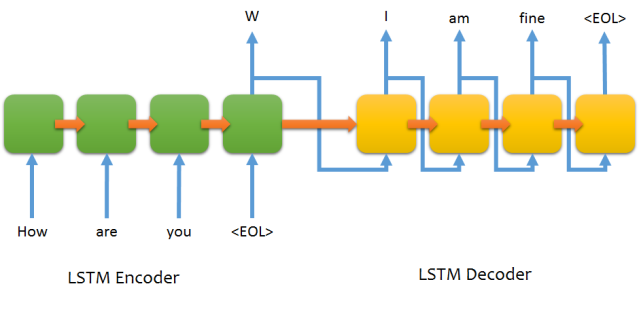
\includegraphics[width=0.8\textwidth]{seq2seq}
\caption{Modelul Sequence-to-Sequence}
\end{figure}

\paragraph{}
Aceast tip de arhitectur\u a este \^ impar\c tit\u a \^ in dou\u a jum\u at\u a\c ti: codor (encoder) \c si decodor (decoder). Sarcina codorului este s\u a primeasc\u a o fraz\u a cu un num\u ar variabil de cuvinte ca intrare iar unica sa ie\c sire \footnote{Ie\c sirea ultimului element din secven\c t\u a} s\u a fie o captur\u a a \^ intregii intrari (un vector de lungime fix\u a). Aceast\u a captur\u a poate fi privit\u a ca o sumarizare a \^ intregii fraze. Sarcina decodorului este de a \^ inv\u a\c ta fraze pornind de la ie\c sirea codorului, care va deveni prima intrare din decodor, \c si restul intrarilor precedente. Intrarea curent\u a \(w_{n}\) \^ in decodor este ie\c sirea de la timpul anterior, \(w_{n-1}\). Modelarea se transform\u a astfel \^ intr-o probabilitate condi\c tionat\u a: \(P(w_{n} | w_{1}, w_{2},..., w_{n-1}, c)\), unde \(c\) reprezint\u a ie\c sirea codorului, deseori \^ int\^ alnit sub numele de context \^ in literatura de specialitate.

\paragraph{}
Intr\u arile \^ in acest model sunt de forma \^ intrebare-r\u aspuns. Original folosit ca model de transla\c tie, unde intrarea pentru codor era fraza \^ intr-o limb\u a iar intrarea \^ in decodor era fraza tradus\u a \^ in limba dorit\u a, acest principiu se poate aplica la fel de u\c sor pentru a modela o conversa\c tie. Spre deosebire de traducere unde totul se \^ int\^ ampla punctual iar r\u aspunsul nu depinde dec\^ at de intrarea curent\u a, o conversa\c tie este foarte dependent\u a de un context. F\u ar\u a acest context, partenerul angrenat \^ in discu\c tie ar r\u aspunde mereu lu\^ and \^ in considerare doar ce i s-a spus \^ in momentul de fa\c t\u a, ignor\^ and orice replic\u a anterioar\u a. Acesta nu este un comportament dorit \^ in cadrul unei conversa\c tii \c si de aceea modelul seq2seq nu este destul de puternic de sine st\u at\u ator pentru a modela o discu\c tie.

\section{Hierarchical Recurrent Encoder-Decoder}

\paragraph{}
Modelarea contextului discu\c tiei reprezint\u a una dintre principalele nevoi \^ in ceea ce prive\c ste o conversa\c tie care dore\c ste s\u a par\u a c\^ at mai real\u a. P\^ an\u a recent, cea mai apropiat\u a arhitectur\u a care realiza acest lucru era modelul seq2seq, \^ ins\u a contextul era re\c tinut doar la nivelul unei singure fraze. \^ In anul 2016, Iulian \c Serban et Al. a introdus re\c teaua Hierarchical Recurrent Encoder-Decoder (HRED - Figura 3.4). Ea poate fi vazut\u a ca o extensie peste seq2seq. Avantajul acesteia este c\u a poate re\c tine contextul discu\c tiei.

\begin{figure}[H]
\centering
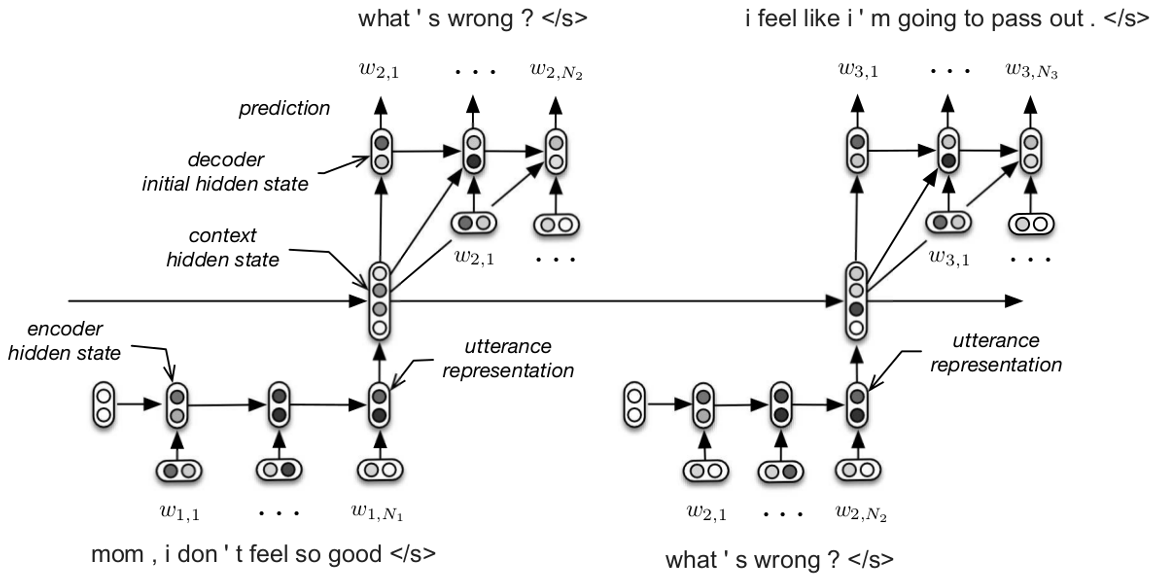
\includegraphics[width=1\textwidth]{hred}
\caption{Hierarchical Recurrent Encoder-Decoder}
\end{figure} 

\paragraph{}
Dup\u a cum se poate observa, modelul este construit prin al\u aturarea mai multor re\c tele seq2seq legate \^ intre ele printr-o RNAR contextual\u a. Dup\u a cum sugereaz\u a \c si numele, rolul acestei RNAR este de a re\c tine contextul discu\c tiei de-a lungul mai multor fraze. Spre deosebire de seq2seq, ie\c sirea codorului nu mai este oferit\u a direct ca \c si prim\u a intrare pentru decodor, aceasta trec\^ and mai \^ intai prin RNAR contextual\u a. Pentru a fi mai u\c sor de \^ inteles ce se \^ intampl\u a, ne putem imagina toate cele \(n\) codoare \c si decodoare ca fiind simple unit\u a\c ti de intrare, respectiv ie\c sire \^ intr-o RNAR obi\c snuit\u a. Precum sunt \^ intr-o RNAR ie\c sirile dependente at\^ at de intrarea curent\u a, c\^ at \c si de cele precedente, prin analogie putem deduce c\u a \^ intr-o re\c tea HRED, fiecare ie\c sire depinde de fraza curent\u a \c si de contextul discu\c tiei (frazele precedente).

\subsection{Celula GRU}

\paragraph{}
Gated Recurrent Unit sau GRU este un tip de celul\u a pentru o RNAR, menit\u a s\u a o \^ inlocuiasc\u a pe cea LSTM. Ecua\c tiile din spatele celulei(3.2) sunt asem\u an\u atoare cu cele LSTM.

\begin{equation}
\begin{split}
z = \sigma(x_{t}U^{z} + s_{t-1}W^{z})\\
r = \sigma(x_{t}U^{r} + s_{t-1}W^{r})\\
h = \tanh(x_{t}U^{h} + (s_{t-1} \circ r)W^{h})\\
s_{t} = (1 - z) \circ h + z \circ s_{t-1}\\
\end{split}
\end{equation}

GRU are doar dou\u a por\c ti: poarta \(r\) de resetare (reset gate) \c si poarta \(z\) de actualizare (update gate). Intuitiv, poarta de resetare determin\u a cum se va combina noua intrare cu memoria precedent\u a iar cea de actualizare define\c ste c\^ at de mult\u a memorie anterioar\u a se p\u astreaz\u a. Principalele diferen\c te \^ intre GRU \c si LSTM sunt:
\begin{itemize}
  \item GRU are doar dou\u a por\c ti, pe c\^ and LSTM trei.
  \item GRU nu posed\u a o memorie intern\u a \(c_{t}\) care s\u a fie diferit\u a de starea ascuns\u a expus\u a. Nu con\c tine poarta de ie\c sire care este prezent\u a pentru LSTM.
  \item Poarta de intrare \c si cea de ie\c sire sunt cuplate de poarta de actualizare, iar poarta de resetare este aplicat\u a direct st\u arii ascunse anterioare. Astfel, responsabilitatea por\c tii de resetare din LSTM este \^ imp\u ar\c tit\u a \^ intre cea de resetare \c si cea de actualizare de la GRU.
  \item Nu se aplic\u a o a doua neliaritate atunci c\^ and se calculeaz\u a ie\c sirea.
\end{itemize}

Nu exist\u a o arhitectur\u a c\^ a\c stig\u atoare clar\u a \^ intre LSTM \c si GRU. Av\^ and mai pu\c tini parametri (\(U\) \c si \(W\)), GRU se antreneaz\u a mai rapid \c si are nevoie de mai pu\c tine date pentru a generaliza. Pe de alt\u a parte, o cantitate mare de date	exprim\u a o putere mai mare de modelare din partea LSTM \c si astfel se pot ob\c tine rezultate mai bune. Pentru realizarea acestei aplica\c tii a fost aleas\u a o arhitectur\u a de tip GRU.

\subsection{HRED bidirec\c tional}

\paragraph{}
Rolul codorului, precum a fost men\c tionat mai devreme, este s\u a captureze informa\c tia unei fraze \^ intr-un vector de lungime fix\u a. \^ In orice limbaj, sensul unui cuv\^ ant nu este stabilit doar de cuvintele precedente ci \c si de cele ce vor urma. Deoarece RNAR modeleaz\u a cuvintele dintr-o fraz\u a pornind de la cuv\^ antul \(w_{1}\) la \(w_{n}\), \^ in\c telesul din viitor al acestora este ignorat, iar captura frazei poate s\u a nu fie \^ indeajuns de reprezentativ\u a. Astfel, este propus\u a folosirea unei RNAR bidirec\c tionale (Figura 3.5) pentru codor. Acest tip de re\c tea folose\c ste dou\u a parcurgeri ale secven\c tei de intrare: cea \^ inainte, care se desf\u a\c soar\u a \^ in mod obi\c snuit \c si cea invers\u a (de la \(w_{n}\) la \(w_{1}\)), pentru capturarea \^ in\c telesului din viitor al cuvintelor. Ie\c sirea pentru pargurgerea \^ inainte va fi la timpul \(n\) iar cea pentru parcurgerea invers\u a va fi la timpul ini\c tial. Vectorul de lungime fix\u a va fi format din concatenarea celor dou\u a ie\c siri ale re\c telei bidirec\c tionale.

\begin{figure}[H]
\centering
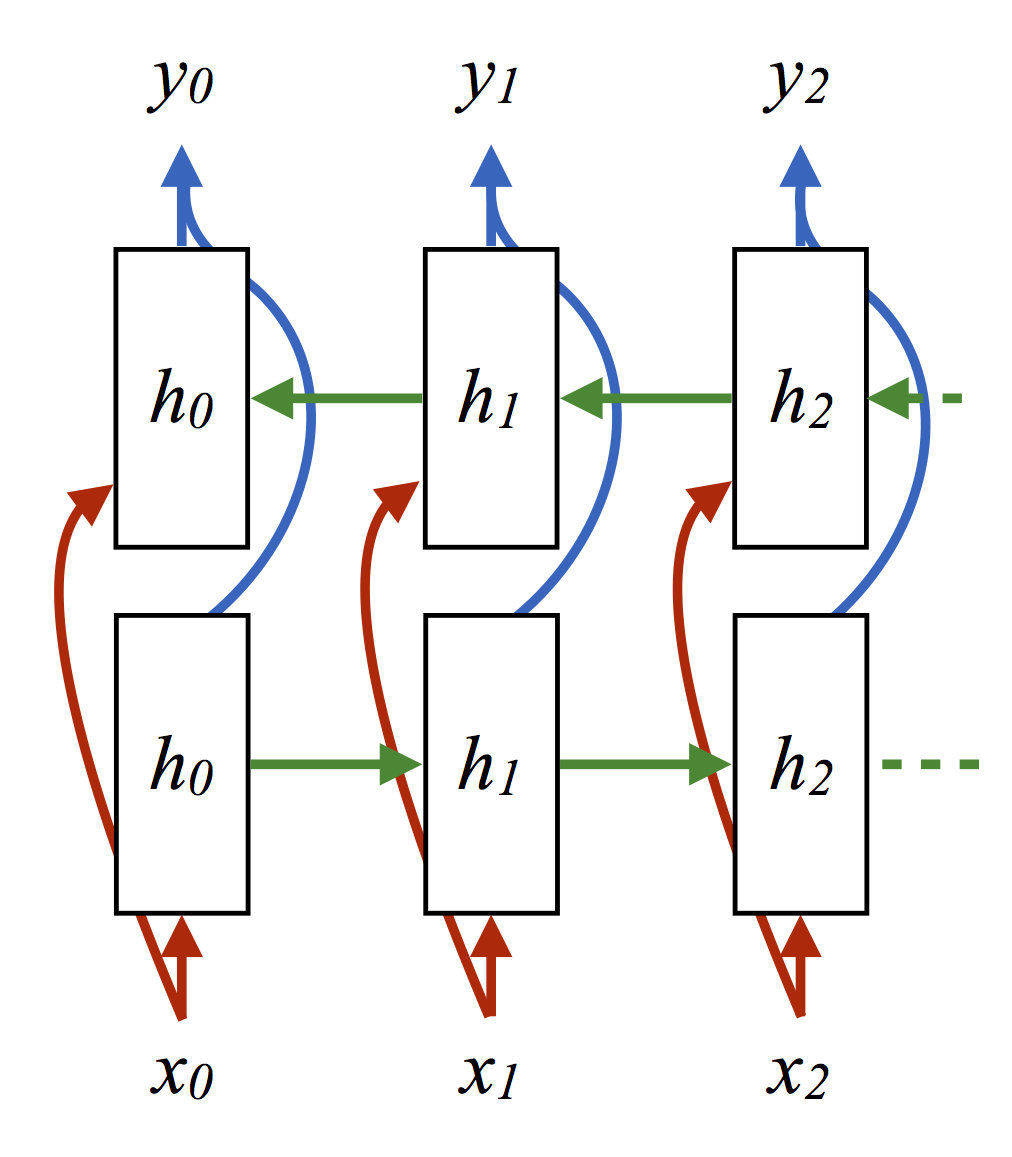
\includegraphics[width=0.5\textwidth]{bidirectional_rnn}
\caption{RNAR bidirec\c tional\u a}
\end{figure} 

\section{Word Embeddings}

\paragraph{}
Buna reprezentare a caracteristicilor unei intr\u ari conduce la rezultate comparativ mai bune fa\c t\u a de situa\c tiile unde acestea sunt \^ inf\u aptuite manual. C\^ and vine vorba despre procesarea natural\u a de limbaj, buna reprezentare a cuvintelor din vocabular (word embeddings) \^ inseamn\u a un factor decisiv pentru succesul final. O reprezentare evident\u a ar fi folosirea codific\u arii de tipul one-hot care presupune un vector de lungimea vocabularului, umplut cu elemente \(0\) iar pozi\c tia pe care se afl\u a cuv\^ antul va fi marcat\u a cu \(1\). Dac\u a lungimea vocabularului este mare, vectorul va deveni rar (sparse) \c si avem de a face cu no\c tiunea de blestemul dimensionalit\u a\c tii\footnote{Dimensionalitatea vectorului de intrare este extrem de mare iar arhitectura re\c telei nu este capabil\u a s\u a modeleze distribu\c tia de probabilit\u a\c ti a datelor}. Astfel, este necesar\u a o codificare compact\u a, mai inteligent\u a, care s\u a fie de asemenea semnificativ\u a pentru semantica cuvintelor.

\subsection{Word2vec}

\paragraph{}
\^ In anul 2013, Mikolov et al. a propus un model pentru word embeddings care se nume\c ste word2vec. \^ In prezent, atunci c\^ and vine vorba despre modelare de limbaj natural, word2vec este solu\c tia cea mai abordat\u a \^ in practic\u a. Aceasta propune folosirea unor vectori de lungime fix\u a, compact\u a care totodat\u a s\u a captureze sensul cuvintelor. Ideea de baz\u a este ca \^ in spa\c tiul n-dimensional folosit, cuvintele cu semantic\u a asem\u anatoare s\u a aib\u a un scor de similaritate c\^at mai mare. Ca \c si metric\u a de similaritate preferat\u a pentru cuantificarea asem\u an\u arii \^ intre reprezentarea a dou\u a cuvinte, c\^ astig\u atoarea este de cele mai multe ori similaritatea cosinus (ecua\c tia 3.3). Cel mai popular exemplu produs pentru a descrie puterea de modelare folosit\u a de word2vec este \(king - man + woman \approx queen\). Figura 3.6 captureaz\u a ideea de word2vec vizualizat \^ intr-un spa\c tiu bidimensional.

\begin{equation}
s(w_{1}, w_{2}) = \frac{\sum_{i=1}^{n}w_{1i}w_{2i}}{\sqrt{\sum_{i=1}^{n}w_{1i}^{2}}\sqrt{\sum_{i=1}^{n}w_{2i}^{2}}}
\end{equation}

\begin{figure}[H]
\centering
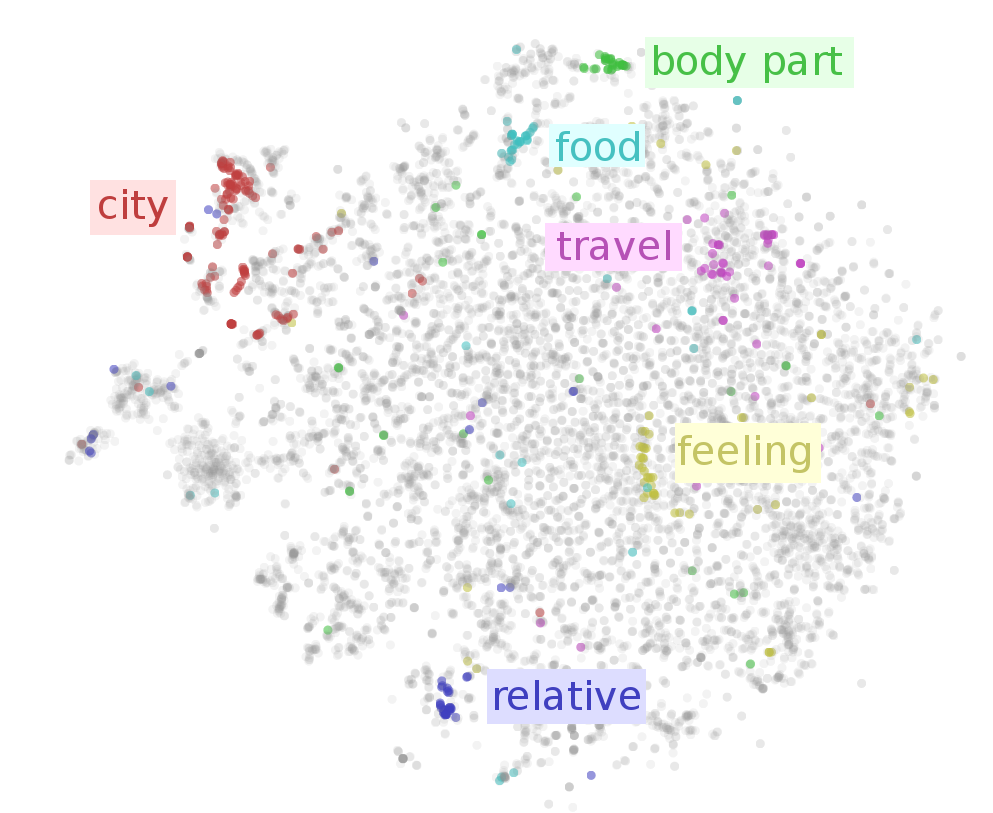
\includegraphics[width=0.7\textwidth]{word_embeddings}
\caption{Word2vec vizualizat \^ in spa\c tiu 2D}
\end{figure} 

\subsection{Word embeddings preantrenate}

\paragraph{}
\^ In machine learning, de cele mai multe ori exist\u a arhitecturi deja antrenate pentru diverse sarcini precum clasificare de imagini, recunoa\c stere vocal\u a etc. La fel este cazul \c si pentru word embeddings. Google a produs o antrenare pe un set de date care const\u a din miliarde de articole de \c stiri, rezult\^ and \^ in urma acesteia word embeddings pentru aproximativ trei miliarde de cuvinte. Dac\u a se dore\c ste antrenarea unei re\c tele care s\u a \^ inve\c te word embeddings pornind de la zero este posibil, \^ ins\u a sarcina este destul de dificil\u a iar rezultatul produs este dependent de natura cuvintelor din setul de date disponibil. Modelarea ideal\u a ar fi ca aceste reprezent\u ari ale cuvintelor s\u a exprime c\^ at mai bine realitatea \^ inconjur\u atoare \c si nu un subset al acesteia. Din acest motiv, este preferat\u a folosirea modelului preantrenat de word embeddings pus\u a la dispozi\c tie de Google.

\section{Predic\c tie}

\paragraph{}
Av\^ and modelul antrenat, acesta trebuie folosit pentru predic\c tie, adic\u a generarea unor r\u aspunsuri adecvate pentru contextul discu\c tiei. Generarea cuvintelor este condi\c tionat\u a at\^ at de context, c\^ at \c si de cuvintele anterior generate. Spre deosebire de antrenare, \^ in momentul predic\c tiei, secve\c ta de ie\c sire este goal\u a ini\c tial (un vector de zerouri). Cuvintele sunt generate secven\c tial, unul c\^ ate unul \c si ad\u augate pe pozi\c tia \(t\) la care a ajuns secven\c ta. Deoarece stratul softmax al secven\c tei de ie\c sire returneaz\u a un vector de probabilit\u a\c ti peste toate cuvintele din vocabular, pentru a returna cuv\^ antul dorit se alege cel cu probabilitatea cea mai mare. Pornind de la aceast\u a idee, exist\u a dou\u a variante de generare: metoda greedy \c si beam search.

\subsection{Greedy}

\paragraph{}
Precum \^ in teoria clasic\u a a algoritmicii, scopul metodelor greedy este s\u a selecteze la fiecare pas optimul local. \^ In cazul de fa\c t\u a, optimul local reprezint\u a cuv\^ antul cu probabilitatea de apari\c tie cea mai mare. Prin acest\u a metod\u a nu este garantat la final c\u a fraza produs\u a este cea mai bun\u a cu putin\c t\u a, deoarece o alt\u a combina\c tie de cuvinte poate produce oric\^ and o fraz\u a cu un scor mai bun\footnote{De regul\u a se utilizeaz\u a media aritmetic\u a a sumei din logaritmul probilit\u a\c tilor cuvintelor frazei}. Astfel, singurul avantaj al acestei metode este viteza de predic\c tie rapid\u a. \^ In practic\u a, se prefer\u a folosirea unor algoritmi mai complexi, capabili s\u a aleag\u a fraza cea mai potrivit\u a dintr-un set de fraze canditat.

\subsection{Beam search}

\paragraph{}
Algoritmul beam search folose\c ste ideea de arbore de c\u autare pentru a genera fraze (Figura 3.6). \^ In locul alegerii cuv\^ antului cu probabilitatea cea mai mare la fiecare pas, se vor alege top \(k\) cuvinte cu cele mai mari probabilit\u a\c ti. \^ In literatur\u a, \(k\) se mai nume\c ste \c si beam size. Fiecare nod (cuv\^ ant) ales va produce un num\u ar \(n_c\) de copii. \^ In felul acesta este garantat\u a generarea mai multor fraze canditat din care se va alege. Fiecare fraz\u a are un scor \(S(f)\), care este de forma ecua\c tiei 3.3, unde \(P(w_{i})\) reprezint\u a probabilitatea cuv\^ antului ales. O fraz\u a devine canditat atunci c\^ and cuv\^ antul curent generat este simbolul de sf\^ ar\c sit de propozi\c tie. \^ In momentul \^ in care algoritmul a terminat de generat toate frazele canditat, cea mai bun\u a este determinat\u a ca fiind cea cu scorul \(S(f)\) cel mai mare.\\

\begin{equation}
\begin{split}
S(f) = \frac{1}{n} \sum_{i=0}^{n} \log P(w_{i})
\end{split}
\end{equation}

\paragraph{}
Pentru ca acest arbore de c\u autare s\u a nu capete o cre\c stere exponen\c tial\u a, la fiecare pas se p\u astreaz\u a un numar egal cu beam size cele mai bune fraze iar restul sunt decartate. Acest algoritm nu asigur\u a de departe optimul global, \^ ins\u a spa\c tiul c\u aut\u arii oferit de folosirea unui arbore este mult mai bine dezvoltat \c si ales dec\^ at la metoda greedy. Cu c\^ at beam size si num\u arul de copii genera\c ti sunt mai mari, cu at\^ at algoritmul ofer\u a solu\c tii c\^ at mai apropiate de optimul global. De asemenea, odat\u a cu cre\c sterea acestor parametri, cre\c ste \c si timpul de c\u auture \c si generare \^ in arbore. De aceea, trebuie s\u a existe un compromis \^ intre calitatea predic\c tiei \c si viteza de execu\c tie a algoritmului.

\begin{figure}[H]
\centering
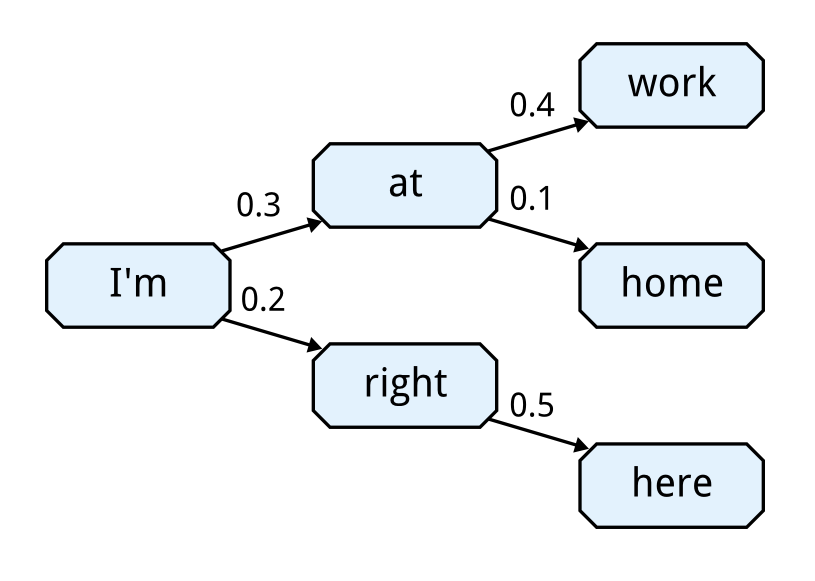
\includegraphics[width=0.6\textwidth]{beam_search}
\caption{Arbore de c\u autare pentru algoritmul beam search}
\end{figure} 

\section{Cross entropy}

\paragraph{}
TODO